\documentclass{article}

\usepackage{url}
\usepackage{amsmath,amssymb}
\usepackage{setspace}
\usepackage{verbatim}
\usepackage{graphicx} %subfigure
\usepackage{caption} % subfigure
\usepackage{subcaption}  %subfigure
\usepackage{listings}
\usepackage[usenames,dvipsnames]{color}
\usepackage[margin=.8in]{geometry}
\usepackage{indentfirst}
\setlength{\parindent}{0mm}
\setlength{\parskip}{0mm}
\usepackage{multirow}
\usepackage{placeins}

\title{STA 250, Lab 1}
\author{Longphi Nguyen\\ \\}
\setcounter{secnumdepth}{0}

\begin{document}
\section{Problem 2}
\begin{table}[!ht]
\centering
\begin{tabular}{|rrr|}
\hline
& beta\_0 & beta\_1 \\  
\hline
p\_01 & 0.01 & 0.01 \\  
p\_05 & 0.07 & 0.03 \\  
p\_10 & 0.10 & 0.07 \\  
p\_25 & 0.23 & 0.20 \\  
p\_50 & 0.51 & 0.47 \\  
p\_75 & 0.75 & 0.73 \\  
p\_90 & 0.89 & 0.88 \\  
p\_95 & 0.94 & 0.95 \\  
p\_99 & 0.99 & 1.00 \\  
\hline
\end{tabular}
\caption{Coverage Summaries}
\end{table}

\begin{figure}[!ht]
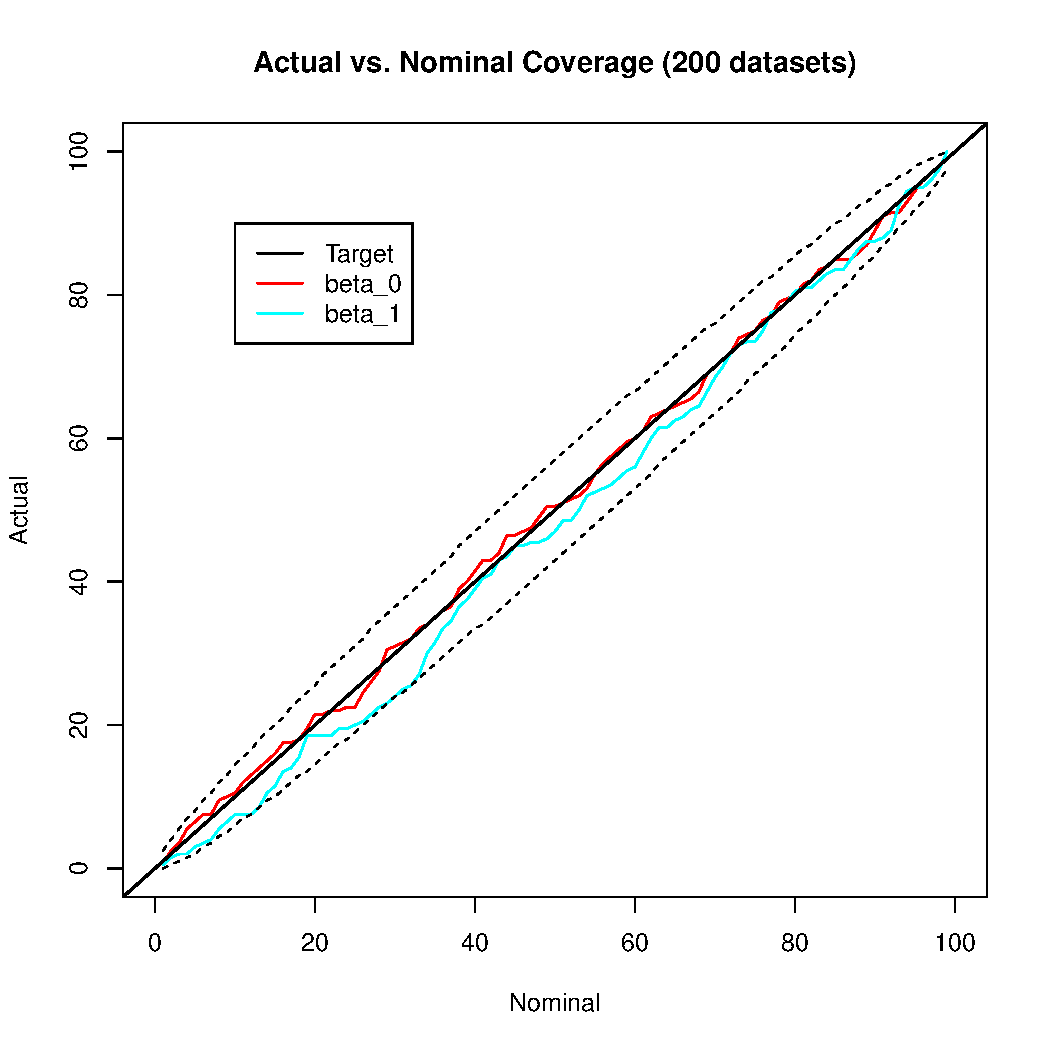
\includegraphics[width=.8\textwidth]{coverage_line_plot}
\caption{Coverage Line PLot}
\end{figure}

\FloatBarrier
\section{Problem 3}

Note that for this problem, the number of iterations used was 30000 and the burnin period was 5000 iterations with retuning every 500 iterations.

\subsection{Lag-1 Autocorrelation}
\begin{table}[!ht]
\centering
\begin{tabular}{|r|rrrrrrrrrrr|}
\hline
& 1 & 2 & 3 & 4 & 5 & 6 & 7 & 8 & 9 & 10 & 11 \\ 
\hline
1 & 1.00 & -0.87 & -0.06 & 0.10 & -0.02 & -0.00 & 0.27 & 0.21 & -0.16 & -0.14 & -0.22 \\ 
2 & -0.87 & 0.99 & -0.02 & -0.03 & 0.02 & 0.08 & -0.29 & -0.27 & 0.07 & 0.13 & 0.14 \\ 
3 & -0.06 & -0.02 & 0.98 & -0.20 & -0.15 & -0.58 & -0.19 & 0.00 & -0.04 & -0.09 & -0.04 \\ 
4 & 0.10 & -0.03 & -0.20 & 0.99 & -0.42 & 0.05 & -0.14 & -0.12 & -0.43 & 0.01 & 0.04 \\ 
5 & -0.02 & 0.02 & -0.16 & -0.41 & 0.96 & -0.30 & -0.04 & 0.10 & 0.39 & -0.13 & 0.10 \\ 
6 & -0.00 & 0.08 & -0.58 & 0.05 & -0.31 & 0.98 & 0.21 & 0.05 & -0.25 & -0.03 & -0.04 \\ 
7 & 0.27 & -0.29 & -0.20 & -0.14 & -0.04 & 0.22 & 0.94 & -0.57 & 0.08 & -0.01 & 0.01 \\ 
8 & 0.21 & -0.27 & 0.00 & -0.12 & 0.10 & 0.05 & -0.57 & 0.99 & 0.10 & 0.05 & 0.09 \\ 
9 & -0.16 & 0.07 & -0.04 & -0.43 & 0.39 & -0.24 & 0.08 & 0.10 & 0.88 & -0.19 & 0.29 \\ 
10 & -0.14 & 0.13 & -0.09 & 0.01 & -0.12 & -0.03 & -0.01 & 0.05 & -0.19 & 0.97 & 0.17 \\ 
11 & -0.22 & 0.13 & -0.04 & 0.04 & 0.10 & -0.04 & 0.01 & 0.09 & 0.29 & 0.17 & 0.77 \\ 
\hline
\end{tabular}
\caption{Lag-1 autocorrelation for each $\beta$.}
\end{table}

\subsection{Related Variables}
Table \ref{breastQuantiles} shows the quantiles of the sample obtained through Metropolis Hastingsfor the breast cancer dataset. The incidence matrix was normalized (each column made to have mean of 0 and variance of 1). So, from the Table \ref{breastQuantiles}, we can say that variables 2, 3, and 6 seem to be not related to cancer diagnosis, since the (5\%, 95\%) quantiles for those variables contain 0. Similarly, the (5\%, 95\%) quantiles for the other variables do not contain 0, so they seem to be related to cancer diagnosis.

That is, (area, compactness, fracdim) seem to not be related to cancer diagnosis, while (concavepts, concavity, perimeter, radius, smoothness, symmetry, texture), do seem to be related to cancer diagnosis. 

\begin{table}[!ht]
\centering
\begin{tabular}{|r|rrrrrrrrrrr|}
\hline
quantile & 1 & 2 & 3 & 4 & 5 & 6 & 7 & 8 & 9 & 10 & 11 \\ 
\hline
1 & -1.36 & -1.14 & -1.58 & 0.15 & 0.04 & -1.65 & -0.37 & -0.03 & 0.13 & -0.16 & 0.89 \\
5 & -1.18 & -0.79 & -1.27 & 0.57 & 0.36 & -1.32 & 0.14 & 0.42 & 0.38 & .007 & 1.05 \\
10 & -1.06 & -.61 & 1.03 & 0.811 &0.54 & -1.14 & 0.43 & 0.66 & 0.51 & 0.09 & 1.13 \\
90 & -0.18 & 0.38 & 0.45 & 2.56 & 1.75 & 0.07 & 2.51 & 2.65 & 1.43 & 0.78 & 1.75 \\
95 & -0.03 & 0.49 & 0.68 & 2.80 & 1.91 & 0.24 & 2.76 & 2.96 & 1.57 & 0.88 & 1.85 \\
99 & 0.25 & 0.68 & 1.14 & 3.3 & 2.23 & 0.59 & 3.17 & 3.55 & 1.83 & 1.07 & 2.02 \\
\hline
\end{tabular}
\caption{Quantiles for each $\beta$, with variable 1 being the intercept.}
\label{breastQuantiles}
\end{table}

\subsection{Posterior Predictive Check}

The posterior predictive check was done using the mean and 30000 repitions. It should be expected that the probability of the sample mean being greater than the real mean should be about 0.5, by definition of the mean. The values, shown in Table \ref{probabilities}, agree with this.

\begin{table}[!ht]
\centering
\begin{tabular}{|rrrrrrrrrrrr|}
\hline
& 1 & 2 & 3 & 4 & 5 & 6 & 7 & 8 & 9 & 10 & 11\\
\hline
& 0.50445 & 0.49588 & 0.50164 & 0.49946 & 0.49949 & 0.49776 & 0.50022 & 0.50242 & 0.50145 & 0.49809 & 0.49971 \\
\hline
\end{tabular}
\caption{P(sample mean $>$ actual mean) for the 11 variables}
\label{probabilities}
\end{table}

\FloatBarrier
\newpage

\section{BLR\_functions.R}

\begin{verbatim}
library(coda) # for mcmc object

# % Sample new theta using normal distribution centered around each element
propose<-function(theta.prop, v)
{
# Note for non-R users: "invisible" can be used like a "return" statement
# if it's the last line of the function
	invisible(rnorm(length(theta.prop), mean=theta.prop, sd=v))
}

# % Calculate posterior
posterior<-function(theta.post, m, y, mu=0, sigma=1)
{
# Calculate logit^-1. The if statements are error checks
# (e.g. R gives exp(*)=NA if it is too large)
	try(z<-exp(X%*%theta.post))
		if(exists("z")==FALSE || class(z)=="try-error" || is.infinite(z)
				|| is.na(z)) return(NA)
			ex=z/(1+z)
				if(exists("ex")==FALSE || class(ex)=="try-error" || is.infinite(ex)
						|| is.na(ex)) return(NA)

# and take the log of the posterior
					invisible(sum(log(ex^y * (1-ex)^(m-y)))
							+sum(log(dnorm(theta.post, mu, sigma))))
# Below is proportionally the same, but avoid having to fully calculate
# dbinom. In particular, the factorials, so the above is slightly faster.
#	return(sum(log(dbinom(y, m, ex)))+sum(log(dnorm(theta.post, mu, sigma))))
}

# % Calculate proposal distribution (a normal distr. in this case)
proposal<-function(theta1, theta2)
{
	invisible(dnorm(theta2, mean=theta1, sd=v))
}

# % Only useful for weird reasons.
thetat<-function(theta, j)
{
	temp=theta[1,]
		temp[j]=theta[2,j]
		invisible(temp)
}

# % The meaty stuff.
"bayes.logreg" <- function(m, y, X, beta.0, Sigma.0.inv,
		niter=30000, burnin=10000,
		print.every=500, retune=500,
		verbose=TRUE)
{
# --==| Initialization |==--
	p=length(beta.0)
		v=sqrt(diag(Sigma.0.inv)) # vector of standard deviation for parameter j

# initialize matrix of sample at iteration i for parameter j
		theta=matrix(NA, ncol=p, nrow=niter+burnin)
		theta[1,]=beta.0

# initialize matrix of acceptance rate at iteration i for parameter j
		acceptance=matrix(NA, ncol=p, nrow=niter+burnin)
		acceptance[1,]=rep(.5,length(beta.0))
		printIt=print.every # iteration counter; prints when == 0
		retuneIt=retune # iteration counter; retunes when == 0


# --==| Start Metropolis Hastings |==--
		for(i in 2:(burnin+niter))
		{
			posteriorBeta = posterior(theta[i-1,], m, y)
				theta[i,] = theta.star = propose(theta[i-1,], v)

				for(j in 1:p)
				{
# Determine acceptance
# Note: Since the proposal is symmetric, I don't bother calculating it,
# so it is commented out.
					alpha=min(log(1), posterior(thetat(theta[(i-1):i,],j), m, y)
							- posteriorBeta) # *proposal(theta.star, theta[[i]][j])
# / proposal(theta[[i]][j], theta.star))
																													 if(is.na(alpha)) alpha<-log(1) # never accept if there was an error
# alpha is in log scale, so acceptance is exp(alpha) 
																														 acceptance[i,j]=exp(alpha)
																															 if(log(runif(1)) < alpha)
																															 {
																																 theta[i,j] = theta.star[j] # accepted!
																																	 if(verbose==TRUE) 
																																		 print(sprintf("[%i, %i, %.2f] accepted with probability %.2f",
																																					 i, j, theta.star[j], acceptance[i,j]))
																															 }else{
																																 theta[i,j] = theta[i-1,j] # rejected!
																															 }
				}


# --==| Retuning if still in the burnin period |==--
			if(i<=burnin && retuneIt==0)
			{
				beta.0=sapply(1:p, function(k) mean(theta[(i-retune+1):i,k]))
																															 for(k in 1:p)
				{
					avgAcceptance = mean(acceptance[i-retune+1, k])
# variances are adjusted based on how far the acceptance rate is,
# targeting the [.3, .5] range. The adjustments are randomized a little.
						if(avgAcceptance<.1) v[k]=v[k]*runif(1, min=.1, max=.2)
						else
							if(avgAcceptance<.3) v[k]=v[k]*runif(1, min=.4, max=.6)
							else
								if(avgAcceptance>.8) v[k]=v[k]*runif(1, 1.7, 1.8)
								else
									if(avgAcceptance>.5) v[k]=v[k]*runif(1, 1.3, 1.6)

				}
				retuneIt=retune
			}


# --==| Printing stuff |==--
			printIt=printIt-1
				retuneIt=retuneIt-1
				if(printIt==0)
				{
					print(sprintf("[estimate] = %s", paste(round(sapply(1:p, function(k)
											mean(theta[1:i,k])), 2), collapse=", ")))
						print(sprintf("[variance] = %s", paste(round(v,2), collapse=", ")))
						print(sprintf("[acceptRate] = %s", paste(round(sapply(1:p, function(k)
												mean(acceptance[(i-retune+1):i, k])), 2), collapse=", ")))
																										 printIt=print.every
				}
		}

	invisible(list(burned=theta[1:burnin,],
				thetas=mcmc(theta[(burnin+1):nrow(theta),]),
				acceptance=acceptance))
}
\end{verbatim}

\end{document}
